\documentclass[a4paper,12pt]{article}
\usepackage{amsfonts}
\usepackage{amsthm}
\usepackage{amsmath}
\usepackage[utf8]{inputenc}
\usepackage[polish]{babel}
\usepackage{polski}
\usepackage{verbatim}
\usepackage{graphicx}

\linespread{1.0}

\newtheorem{defi}{Definicja}
\newtheorem{theo}[defi]{Twierdzenie}
\newtheorem{lemma}[defi]{Lemat}
\newtheorem{obs}[defi]{Obserwacja}

\newcommand{\E}{\mathbb{E}}
\newcommand{\R}{\mathbb{R}}
\newcommand{\RR}{\mathbb{R}^3}
\newcommand{\RRR}{\mathbb{R}^{3 \times 3}}
\newcommand{\RRRq}{\mathbb{R}^{4 \times 4}}
\newcommand{\RRq}{\mathbb{R}^4}
\newcommand{\vecs}[2]{\langle #1 , #2 \rangle}

\newcommand{\vectt}[2]{\begin{bmatrix} #1 \\ #2 \end{bmatrix}}
\newcommand{\vecttt}[3]{\begin{bmatrix} #1 \\ #2 \\ #3 \end{bmatrix}}
\newcommand{\vectttt}[4]{\begin{bmatrix} #1 \\ #2 \\ #3 \\ #4 \end{bmatrix}}
\newcommand{\Vectt}[4]{\begin{bmatrix} #1 & #2 \\ #3 & #4 \end{bmatrix}}

\title{Reprezentacja trójwymiarowej, ruchomej sceny}

\author{M.~K.~Karpiński\\
\\
Uniwersytet Wrocławski\\
Instytut Informatyki}

\date{Wrocław, dnia \today\ r.}

\begin{document}

\maketitle

\section{Wstęp}
\indent \indent Badanie geometrycznych zależności między trójwymiarową sceną a dwuwymiarowymi obrazami generowanymi poprzez ruch kamery po scenie, leży w sercu dwóch fundamentalnych typów przekształceń:

\begin{enumerate}
  \item ruchu Euklidesowego (czyli ruchu brył sztywnych)
  \item rzutu perspektywicznego
\end{enumerate}

Pierwsze z nich zostanie omówione na dzisiejszym seminarium, drugie zaś zostanie omówione za tydzień przez Maćka. Obydwa tematy będą wymagały znajomości podstawowych obiektów i notacji z dziedziny algebry. Tak na prawdę, całe dzisiejsze seminarium, to będzie czysta algebra, ale mam nadzieję, że was tym nie zanudzę. Agenda:

\begin{enumerate}
\item Świat, którym się zajmujemy (przestrzeń $\E^3$)
\item Obiekty, które żyją w tym świecie (bryły sztywne)
\item Ruch obrotowy i jego reprezentacje
\item Reprezenatcje pełnego ruchu bryły sztywnej 
\item Przekształcenia współrzędnych i prędkości
\end{enumerate}

\section{Przestrzeń euklidesowa}
\indent \indent Niech $\E^3$ będzie trójwymiarową przestrzenią euklidesową. Jest to naturalny sposób modelowania świata rzeczywistego. W ogólnym przypadku przestrzeń euklidesowa zdefiniowana jest poprzez 5 aksjomatów Euklidesa:

\begin{itemize}
\item dowolne dwa punkty można połączyć odcinkiem
\item dowolny odcinek można przedłużyć nieograniczenie, uzyskując prostą
\item dla danego odcinka można zaznaczyć okrąg o środku w jednym z jego końców i promieniu równym jego długości
\item wszystkie kąty proste są przystające
\item dwie proste, które przecinają przecią w taki sposób, że suma kątów wewnętrzych po jednej stronie jest mniejsza od dwóch kątów prostych, przetną się z tej właśnie strony
\end{itemize}

Dla naszych potrzeb, trójwymairową przestrzeń euklidesową będziemy reprezentować za pomocą układu współrzędnych kartezjańskich: każdy punkt $p \in \E^3$ może być zidentyfikowany poprzez punkt w $\R^3$:

\begin{equation}
X = [x_1, x_2, x_3]^T = 
\begin{bmatrix}
x_1 \\ x_2 \\ x_3
\end{bmatrix}
\in \RR
\end{equation}


Zamiast $x_1,x_2,x_3$ często będziemy pisać $x,y,z$. Dzięki temu mamy zależność $1-1$ między $\E^3$ a $\R^3$, więc bezpiecznie możemy mówić o punktach i ich współrzędnych, jakby były tym samym bytem. Przeszliśmy pierwszy krok w stronę mierzenia odległości i kątów. Czego nam brakuje, to związać $\E^3$ z metryką. Precyzyjna definicja metryki opiera się na definicji wektora:

\begin{defi}(wektor)
W przestrzeni euklidesowej, wektor $v$ jest reprezentowany przez parę punktów $p,q \in \E^3$ i zdefiniowany jako strzałka skierowana łącząca $p$ do $q$. Piszemy $v = \vec{pq}$.
\end{defi}

\noindent Wektor $v$ zapisujemy także jako $[v_1,v_2,v_3]^T \in \R^3$, gdzie $v = Y - X$.

Wektor jest zaczeniony, jeśli podamy punkt $p$ explicite. W przeciwnym wypadku mówimy o wektorach swobodnych.

Zbiór wszystkich wektorów swobodnych tworzy liniową przestrzeń wektorową z liniową kombinacją dwóch wektorów $v, u \in \R^3$ zdefiniowaną jako:

\begin{equation}
\alpha v + \beta u = [\alpha v_1 + \beta u_1, \alpha v_2 + \beta u_2, \alpha v_3 + \beta u_3]^T, \quad \forall \alpha,\beta \in \R
\end{equation}

Metryka Euklidesowa dla $\E^3$ jest wtedy zdefiniowana poprzez produkt skalarny na przestrzeni wektorowej $\R^3$.

\begin{equation}
\vecs{u}{v} = u^Tv = u_1v_1 + u_2v_2 + u_3v_3, \quad \forall u,v \in \R^3
\end{equation}

Niektóre własności:

\begin{equation}
\| v \| = \sqrt{\vecs{v}{v}} = \sqrt{v^2_1 + v^2_2 + v^2_3}
\end{equation}

\begin{defi}
Jeśli $\vecs{u}{v}=0$, wtedy $u$ i $v$ są ortogonalne.
\end{defi}

Podsumowując: przestrzeń euklidesowa $\E^3$ może być zdefiniowana jako przestrzeń, która identyfikuje się ze zbiorem $\RR$ i posiada metrykę w swojej przestrzeni wektorowej daną poprzez powyższy iloczyn skalarny.

Jeszcze o wektorach: 

\begin{defi}[Iloczyn wektorowy]
Mając dane dwa wektory $u,v \in \R$ ich iloczyn wektorowy (cross product) jest wektorem ze współrzędnymi:
\begin{equation}
  u \times v = 
  \begin{bmatrix}
    u_2v_3 - u_3v_2 \\ u_3v_1 - u_1v_3 \\ u_1v_2 - u_2v_1
  \end{bmatrix}
  \in \RR
\end{equation}
\end{defi}

\noindent Można łatwo sprawdzić, że:

\begin{equation}
\vecs{u \times v}{u} = \vecs{u \times v}{v} = 0, u \times v = -v \times u
\end{equation}

Z tego wynika, że iloczyn wektorowy jest prostopadły do $u$ oraz do $v$ oraz kolejność czynników definiuje zwrot wektora wynikowego. 

Jeśli ustalimy z góry $u$, to iloczyn wektorowy może być reprezentowany przez funkcję z $\RR$ do $\RR$, która bierze $v$ i zwraca $u \times v$. Taka funkcja jest zdefiniowana jako:

\begin{equation}
u \times v = \hat{u}v, \quad \hat{u} = 
\begin{bmatrix}
  0    & -u_3 & u_2  \\
  u_3  & 0    & -u_1 \\
  -u_2 & u_1  & 0
\end{bmatrix}
\in \RRR
\end{equation}

Widać, że $\hat{u}$ jest macierzę antysymetryczną tzn. $\hat{u}^T = -\hat{u}$. Jest oczywiste, że następujący lemat zachodzi:

\begin{lemma}
Macierz $M \in \RRR$ jest antysymetryczna wtedy i tylko wtedy, gdy $M=\hat{u}$ dla pewnego $u \in \RR$
\end{lemma}

Dzięki czemu przestrzeń wektorowa $\RR$ i przestrzeń wszystkich macierzy antysymetrycznych $3 \times 3$ (zwana $so(3)$) są izomorficzne.

\section{Ruch bryły sztywnej}

\indent \indent Wyobraźmy sobie obiekt ruszający się przed kamerą. Aby precyzyjnie zdefiniować jego ruch powinniśmy ustalić trajektorię każdego punktu leżącego na obiekcie. Np. specyfikując współrzędne punktu poprzez funkcję od czasu $X(t)$. Na nasze szczęście nie musimy specyfikować ruchu każdego punktu. Jak za chwilę się przekonamy, do zdefiniowania ruchu obiektu wystarczy ustalić ruch jednego punktu oraz ruch trzech osi współrzędnych zaczepionych w tym punkcie. Powodem tego jest to, że dla każdej bryły sztywnej, odległość między dwoma dowolnymi punktami leżącymi na tej bryle nie zmienia się w czasie podczas ruchu tej bryły. Więc jeśli $X(t)$ i $Y(t)$ są współrzędnymi dowolnych dwóch punktów $p$ i $q$, odległość między tymi punktami jest stała:

\begin{equation}
\| X(t) - Y(t) \| == constant, \quad \forall t \in R
\end{equation}

Ruch bryły sztywnej (lub transformacja bryły sztywnej) jest rodziną funkcji, które określają w jaki sposób współrzędne każdego punktu na bryle sztywnej zmieniają się w czasie (respektując powyższą zasadę). Zdefiniujmy taką funkcję jako:

\begin{equation}
g(t): \RR \rightarrow \RR; X \rightarrow g(t)(X).
\end{equation}

Zamiast patrzeć na całą ciągłą ścieżkę ruszającego się obiektu, skoncentrujemy się na funkcji między jego początkową a końcową konfiguracją (rigid-body displacement) zdefiniowaną jako:

\begin{equation}
g: \RR \rightarrow \RR; X \rightarrow g(X).
\end{equation}

Oprócz transformacji na współrzędnych punktu, $g$ można również wykorzystać do transformacji na wektorach. Niech $v$ będzie wektorem zdefiniowanym przez punkty $p$ i $q$ o współrzędnych $v = Y - X$. Wtedy, po transformacji $g$, otrzymujemy nowy wektor:

\begin{equation}
u = g_*(v) = g(Y) - g(X)
\end{equation}

Jako że $g$ zachowuje odległości pomiędzy punktami, w oczywisty sposób otrzymujemy $\| g_*(v) \| = \| v \|$ dla każdego swobodnego wektora $v \in \RR$.

Zauważmy, że własność zachowania odległości między punktami nie jest wystarczająca aby poprawnie zdefiniować ruch bryły sztywnej. Np. taka transformacja:

\begin{equation}
f : [x,y,z]^T \rightarrow [x,y,-z]^T
\end{equation}

Zachowuje odległość, ale nie zwrot! Aby w naszej rodzinie wykluczyć tego typu funkcje, wymagamy, aby zachowywać nie tylko odległość, ale też zwrot. Formalnie, oprócz zachowania modułu wektora, musimy także zachować produkt wektorowy.

\begin{defi}[Ruch bryły sztywnej (rigid-body motion)]
Funkcja $g: \RR \rightarrow \RR$ jest ruchem bryły sztywnej wtedy, gdy zachodzą:

\begin{enumerate}
\item $\| g_*(v) \|  = \| v \| , \forall v \in \RR$
\item $g_*(u) \times g_*(v) = g_*(u \times v), \forall u,v \in \RR$
\end{enumerate}

\noindent Zbiór wszystkich takich ruchów nazywamy $SE(3)$.
\end{defi}

Nie jest do końca oczywiste, że powyższa definicja zachowuje kąty między wektorami. Ale można to udowodnić w taki sposób: iloczyn skalarny $\vecs{.}{.}$ definiujemy poprzez moduł $\| . \|$ (polarization identity):

\begin{equation}
\vecs{u}{v} = \frac{1}{4}( \| u+v \|^2 - \| u-v \|^2)
\end{equation}

Więc skoro $\| u+v \| = \| g_*(u)+g_*(v) \|$, to otrzymujemy, że:

\begin{equation}
\vecs{u}{v} = \vecs{g_*(u)}{g_*(v)}, \quad \forall u,v \in \RR
\end{equation}

\noindent Innymi słowy, do definicji ruchu bryły sztywnej można dodać zachowanie iloczynu skalarnego.

W jaki sposób te własności pomagają nam precyzyjnie opisać ruch bryły sztywnej? Fakt, że odległości i zwroty są zachowane przez ruch bryły sztywnej oznacza, że punkty nie mogą ruszać się relatywnie do siebie. Konsekwencją tego faktu jest to, że ruch bryły sztywnej może być opisany przez ruch jednego wybranego punktu na bryle i rotacji układu współrzędnych związanego z tym punktem. Będziemy reprezentowali konfigurację bryły sztywnej związując koratezjański układ współrzędnych (frame) do jakiegoś punktu na obiekcie i śledząc ruch tego układu relytywnie do ustalonego układu współrzędnych świata (uład globalny). World (reference) frame.

Weźmy układ współrzędnych wyznaczony przez trzy ortonormalne wektory $e_1,e_2,e_3 \in \RR$, które spełniają:

\begin{equation}
e^T_ie_j = \delta_{ij} = \left\{
  \begin{array}{l l}
    1 & \quad \text{jeśli $i=j$}\\
    0 & \quad \text{wpw}\\
  \end{array} \right.
\end{equation}

Wektory te są ułożone tak, aby tworzyły prawoskrętny układ: $e_1 \times e_2 = e_3$. Ruch bryły sztywnej $g$ daje nam:

\begin{equation}
g_*(e_i)^Tg_*(e_j) = \delta_{ij}, \quad g_*(e_1) \times g_*(e_2) = g_*(e_3)
\end{equation}

To znacza, że wektory wynikowe $g*(e1),g*(e2),g*(e3)$ wciąż tworzą prawoskrętny ortonormalny układ. Więc bryła sztywna zawsze może być rozpoznawana przez prawoskrętny, ortonormalny układ, który będziemy nazywali 'object coordinate frame' lub 'body coordinate frame' oraz jej ruch może być w całości opisany przez ruch takiego układu.

W szczególności powinniśmy ustalić relację między kamerą a resztą świata. Możemy np. ustalić, że 'world frame' jest związany z obiektem kamery i reszta obiektów porusza się względem niej.


\section{Ruch obrotowy i jego reprezentacje}

\subsection{Reprezentacja obrotu poprzez macierze ortogonalne}

Załóżmy, że mamy bryłę sztywną obracającą się wokół ustalonego punktu $o \in \E^3$. Załóżmy, że w tym punkcie znajduje się też początek układu globalnego $W$. Zaczepimy do $o$ jeszcze jeden układ $C$, będący obracającą się kamerą. Relację między tymi dwoma układami współrzędnych ilustruje poniższy rysunek:

\begin{center}
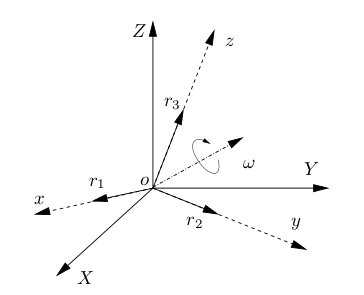
\includegraphics[scale=0.5]{rys1.png}
\end{center}

Konfiguracja układu $C$ względem układu $W$ jest wyznaczona przez współrzędne trzech ortonormalnych wektorów 

\begin{equation}
r_1=g_*(e_1), r_2=g_*(e_2), r_3=g_*(e_3) \in \RR
\end{equation}

$r_1,r_2,r_3$ są po prostu wektorami jednostkowymi położonymi na współrzędnych $x,y,z$ układu $C$. Konfiguracja obracającego się układu jest wtedy w całości wyznaczona przez macierz $3 \times 3$:

\begin{equation}
R_{wc} = [r_1,r_2,r_3] \in \RRR 
\end{equation}

\noindent gdzie $r_1,r_2,r_3$ są ułożone kolumnami. Z tego że $r_1,r_2,r_3$ tworzą układ ortonormalny, mamy:

\begin{equation}
r^T_ir_j = \delta_{ij} = \left\{
  \begin{array}{l l}
    1 & \quad \text{jeśli $i=j$}\\
    0 & \quad \text{wpw}\\
  \end{array} \right.
  \quad \forall i,j \in {1,2,3}
\end{equation}

\noindent co może by zapisane w postaci macierzy:

\begin{equation}
R_{wc}^TR_{wc} = R_{wc}R_{wc}^T = I
\end{equation}

Każda macierz spełniająca powyższą zależność nazywa się macierzą ortogonalną. Z definicji wynika również, że:

\begin{equation}
R_{wc}^{-1} = R_{wc}^T. 
\end{equation}

Z tego że $r_1,r_2,r_3$ tworzą układ prawoskrętny, wymagamy aby wyznacznik macierzy $R_{wc}$ był równy $+1$. Przestrzeń wszystkich takich ortogonalnych macierzy należących do $\RRR$ definiujemy jako:

\begin{equation}
SO(3)=\{ R \in \RRR | R^TR = I, det(R)=+1 \}
\end{equation}

Takie macierze ortogonalne tradycyjnie nazwywają się macierzami rotacji (z wiadomych powodów). (rotation matrices). Side note: $SO(3)$ z operacją mnożenia macierzy tworzą grupę. Dlatego SO(3) nazywa się czasem grupą obrotową. 

\noindent Przykład:

\begin{equation}
R_Z(\theta) = 
\begin{bmatrix}
  1 & 0 & 0 \\
  0 & \cos(\theta) & -\sin(\theta) \\
  0 & \sin(\theta) & \cos(\theta)
\end{bmatrix}
\end{equation}

Wracajac do rysunku, każda macierz obrotu $R_{wc} \in SO(3)$ reprezentuje możliwą konfigurację obiektu obruconego wokół punktu $o$. Ponadto taka macierz reprezentuje transformację z układu współrzędnych $C$ do $W$. Konfigurację ciągle obracającego się obiektu można opisać jako funkcję trajetorii $R(t): t \rightarrow SO(3)$ w przestrzeni $SO(3)$. Jeśli $t \neq 0$, obrót pomiędzy czasem $t_2$ i $t_1$ opiszemy jako $R(t_2,t_1)$. W prosty sposób można wywnioskować iż:

\begin{equation}
R(t_2,t_0) = R(t_2,t_1)R(t_1,t_0) \quad \forall t_0 < t_1 < t_2 \in \R
\end{equation}

\subsection{Reprezentacja obrotu przez współrzędne eksponentne}

Wg autora jest bardziej intuicyjny. Obrót jest parametryzowany poprzez dwie rzeczy:

\begin{itemize}
\item wektor jednostkowy wychodzący z układu
\item kąt obrotu wektora (prawoskrętnie)
\end{itemize}

Wygląda obiecująco, ale czy na pewno można w ten sposób reprezentować każdy obrót bryły sztywnej? Trzeba to udowodnić. Zacznamy od początku.

Mamy trajetorię $R(t): \R \rightarrow SO(3)$, która wyznacza ciągły ruch obrotowy. Obrót musi spełniać warunek:

\begin{equation}
R(t)R^T(t)=I
\end{equation}

Obliczając pochodną w powyższym równaniu po zmiennej $t$ i zauważywszy, że prawa strona jest macierzą stałą, otrzymujemy:

\begin{equation}
\dot{R}(t)R^T(t) + R(t)\dot{R}^T(t)=0 \Rightarrow \dot{R}(t)R^T(t)=-(\dot{R}(t)R^T(t))^T
\end{equation}

Oznacza to, że macierz $\dot{R}(t)R^T(t) \in \RRR$ jest antysymetryczna. Czyli musi istnieć wektor $\hat{\omega}(t) \in \RR$ taki, że:

\begin{equation}
\dot{R}(t)R^T(t) = \hat{\omega}(t)
\end{equation}

\noindent a po pomnożeniu obustronnie przez $R(t)$:

\begin{equation}
\dot{R}(t) = \hat{\omega}(t)R(t)
\end{equation}

Teraz wykorzystamy tą wiedzę do stworzenia użytecznej reprezentacji macierzy rotacyjnej. Zacznijmy od założenia, że $\hat{\omega}$ jest ustalone. Oczywistym jest, że rozwiązanie tego równania jest podane przez:

\begin{equation}
x(t) = e^{\hat{\omega}t}x(0)
\end{equation}

\noindent gdzie $e^{\hat{\omega}t}$ jest eksponentą macierzy:

\begin{equation}
e^{\hat{\omega}t} = I + \hat{\omega}t + \frac{(\hat{\omega}t)^2}{2!} + \cdots + \frac{(\hat{\omega}t)^n}{n!} + \cdots
\end{equation}

Zakładając że $R(0)=I$ jest stanem początkowym rotacji otrzymujemy:

\begin{equation}
R(t) = e^{\hat{\omega}t}
\end{equation}

Aby sprawdzić, czy rzeczywiście $e^{\hat{\omega}t}$ jest macierzą rotacyjną, można wprost z definicji eksponenty pokazać, że:

\begin{equation}
(e^{\hat{\omega}t})^{-1}=e^{-\hat{\omega}t}=e^{\hat{\omega}^Tt}=(e^{\hat{\omega}t})^T
\end{equation}

Czyli $(e^{\hat{\omega}t})^Te^{\hat{\omega}t}=I$. Fizyczna interpretacja $R(t) = e^{\hat{\omega}t}$ jest taka, o której mówiliśmy na początku tego działu, czyli jeśli założymy, że $\| \omega \| = 1$, wtedy $R(t)=e^{\hat{\omega}t}$ jest obrotem dookoła osi $\omega \in \RR$ o kąt $t$ radianów. Ogólnie możemy $t$ absorbować do $\omega$, więc mamy $R = e^{\hat{\omega}}$ dla $\omega$ o dowolnej długości.

Eksponenta definiuje funkcję z przestrzeni $so(3)$ do przestrzeni $SO(3)$, zwie się to ``exponential map''. 

Zauważmy że otrzymaliśmy wzór $R(t) = e^{\hat{\omega}t}$ zakładając, że $\omega(t)$ jest stały. Ale oczywiście nie zawsze tak jest. Wtedy naturalnie powstaje pytanie: czy każda macierz rotacyjna $R \in SO(3)$ może być wyrażona w formie eksponenty? Odpowiedź brzmi: tak, i fakt ten pokazuje poniższe twierdzenie:

\begin{theo}[logarytm SO(3)]
Dla każdego $R \in SO(3)$, istnieje $\omega \in \RR$ takie, że $R = e^{\hat{\omega}}$. 
\end{theo}

\noindent Jest to tzw. funckja z przestrzeni $SO(3)$ do $so(3)$. Zapisujemy $\hat{\omega} = log(R)$

\begin{equation}
R = 
\begin{bmatrix}
  r_{11} & r_{12} & r_{13} \\
  r_{21} & r_{22} & r_{23} \\
  r_{31} & r_{32} & r_{33}
\end{bmatrix}
\end{equation}

\begin{equation}
\theta = \| \omega \| = \arccos(\frac{trace(R)-1}{2})
\end{equation}

\begin{equation}
\omega = \frac{1}{2\sin(\theta)}
\begin{bmatrix}
  r_{32} - r_{23} \\ r_{13} - r_{31} \\ r_{21} - r_{12}
\end{bmatrix}
\end{equation}

Dzięki temu twierdzeniu możemy w efektywny sposób obliczać wektor obrotu mając daną macierz obrotu, ale w jaki sposób efektywnie obliczyć macierz obrotu $R = e^{\hat{\omega}}$ mając dany wektor $\omega$? Z definicji eksponenty to tak nie bardzo. Możemy użyć następującego twierdzenia:

\begin{theo}[wzór Rodrigues'a dla macierzy rotacyjnych]
Mając dany $\omega \in \RR$, eksponenta macierzy $R = e^{\hat{\omega}}$ jest równa:
\end{theo}

\begin{equation}
e^{\hat{\omega}}=I + \frac{\hat{\omega}}{\| \omega \|}\sin(\| \omega \|) + \frac{\hat{w}^2}{\| \omega \|^2}(1 - \cos(\| \omega \|))
\end{equation}

\noindent Wprost z definicji eksponenty możemy zapisać:

\begin{equation}
e^{\hat{\omega}t}= I + \hat{w}(t - \frac{t^3}{3!} + \frac{t^5}{5!} - \cdots) + \hat{w}^2(\frac{t^2}{2!} - \frac{t^4}{4!} + \frac{t^6}{6!} - \cdots)
\end{equation}

\noindent Co w zasadzie kończy dowód.

Oczywiste jest, że jeśli $\| w \|=1$ i $t=2k\pi$, to dostaniemy identyczność ($\forall k$). Więc transformacja z $so(3)$ do $SO(3)$ nie jest bijekcją, bo ma nieskończenie wiele elementów w $SO(3)$.


\section{Reprezentacje pełnego ruchu bryły sztywnej}

\begin{center}
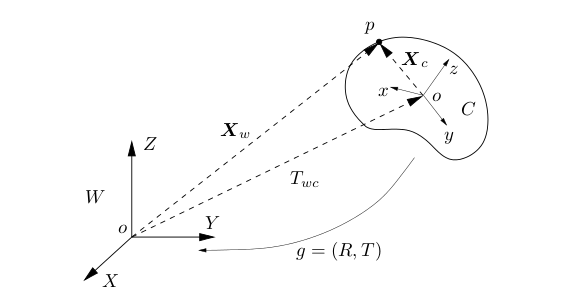
\includegraphics[scale=0.5]{rys2.png}
\end{center}

Czyli ruch z rotacją oraz tranzlacją. Rysunek 3 przedstawia ruszający się obiekt z układem $C$ do niego przypisanym. Aby opisać współrzedne punktu $p$ na obiekcie odnośnie do układu globalnego $W$, jest oczywiste że należy dodać do siebie wektor tranzlacji $T_{wc}$ i wektor $X_c$, ale opisany relatywnie do $W$. Z tego że $X_c$ są współrzędnymi punktu $p$ relatywnymi do układu $C$, mamy $R_{wc}X_c$, gdzie $R_{wc} \in SO(3)$ jest rotacją między układami $W$ i $C$. Wtedy współrzędne $X_w$ można otrzymać tak:

\begin{equation}
X_w = R_{wc}X_c + T_{wc}
\end{equation}

Zwykle będziemy oznaczali pełny ruch bryły sztywnej przez $g_{wc} = (R_{wc},T_{wc})$ lub po prostu $g = (R,T)$ jeśli układy współrzędnych będą w oczywisty sposób wynikały z kontekstu. Wtedy możemy reprezentować na raz rotację i translację pomiędzy dwoma układami współrzędnych. W zwięzłej formie piszemy:

\begin{equation}
X_w = g_{wc}(X_c)
\end{equation}

Zbiór wszsytkich możliwych konfiguracji bryły sztywnej może być opisany przez przestrzeń ruchów brył sztywnych:

\begin{equation}
SE(3) = \{ g = (R,T) | R \in SO(3), T \in \RR \}
\end{equation}

Zauważmy, że $g = (R,T)$ nie jest jeszcze reprezenatcją macierzową dla $SE(3)$. Żeby tak się stało złączenie dwóch ruchów bryły sztywnej musiałoby być iloczynem dwóch macierzy. Aby uzyskać taką reprezentacją musimy wprowadzić pojęcie tzw. współrzędnych jednorodnych.



\subsection{Reprezentacja jednorodna}


\indent \indent Jak niektórzy mogli już zauważyć, w odróżnieniu od samych rotacji obiektów, transformacja pełnego ruchu bryły sztywnej nie jest liniowa, lecz afiniczna. W ramach przypomnienia: powiemy że dwa wektory - $u$ i $v$ - są związane liniową transformacją jeśli $u = Av$ dla pewnej macierzy $A$, i są związane transformacją afiniczną jeśli $u = Av + b$ dla pewnej macierzy $A$ i wektora $b$.

Nie boimy się mimo wszystko, bo możemy dokonać konwersji z transformacji afinicznej do liniowej wykorzystując tzw. współrzędne jednorodne. Zamieniamy punkt $X = [x_1,x_2,x_3]^T \in \RR$ na $\bar{X} = [x_1,x_2,x_3,1]^T \in \RRq$

W efekcie, takie rozszerzenie współrzędnych osadza przestrzeń euklidesową $\E^3$ w hiperpłaszczyźnie $\RRq$ zamiast $\RR$. Współrzędne jednorodne wektora $v = X(q) - X(p)$ są zdefiniowane jako różnica między jednorodnymi współrzędnymi dwóch punktów $q$ i $p$, stąd otrzymujemy:

%\begin{comment}

\begin{equation}
\bar{v} = \begin{bmatrix} v \\ 0 \end{bmatrix} = \begin{bmatrix} X(q) \\ 1 \end{bmatrix} - \begin{bmatrix} X(p) \\ 1 \end{bmatrix} = \begin{bmatrix} v_1 \\ v_2 \\ v_3 \\ 0 \end{bmatrix} \in \RRq
\end{equation}

%\begin{comment}

Zauważmy, że wektory w powyższej formie tworzą podprzestrzeń, w której wszystkie liniowe struktury oryginalnych wektrów $v \in \RR$ są zachowane w niezmienionej formie przez nową reprezentację. Teraz, używając nowej notacji możemy transformację afiniczną $X_w = R_{wc}X_c+ T_{wc}$ przepisać w postaci liniowej:

\begin{equation}
\bar{X}_w = \begin{bmatrix} X_w \\ 1 \end{bmatrix} = \begin{bmatrix} R_{wc} & T_{wc} \\ 0 & 1 \end{bmatrix}\begin{bmatrix} X_c \\ 1 \end{bmatrix} = \bar{g}_{wc}\bar{X}_c
\end{equation}

gdzie macierz $\bar{g}_{wc} \in \RRRq$ zwie się jednorodną reprezentacją ruchu brył sztywnych $g_{wc} = (R_{wc}, T_{wc}) \in SE(3)$. Generalnie, jeśli $g = (R,T)$ wtedy jego reprezentacją jednorodną jest macierz 

\begin{equation}
\bar{g} = \begin{bmatrix} R & T \\ 0 & 1 \end{bmatrix} \in \RRRq
\end{equation}

Zauważmy, że dzięki temu możemy reprezentować transformację współrzędnych bryły sztywnej przez liniowe mnożenie macierzy. Reprezentacja jednorodna $g$ daje nam naturalną macierzową reprezentację $SE(3)$:

\begin{equation}
SE(3) = \{ \bar{g} = \begin{bmatrix} R & T \\ 0 & 1 \end{bmatrix} | R \in SO(3), T \in \RR \} \subset \RRRq
\end{equation}

Używając takiej reprezentacji w łatwy sposób można sprawdzić, że $SE(3)$ spełnia wszystkie wymagania do bycia grupą. W szczególności $\forall g_1,g_2,g \in SE(3)$ mamy:

\begin{equation}
\bar{g}_1\bar{g}_2 = \begin{bmatrix} R_1 & T_1 \\ 0 & 1 \end{bmatrix}\begin{bmatrix} R_2 & T_2 \\ 0 & 1 \end{bmatrix}=\begin{bmatrix} R_1R_2 & R_1T_2+T_1 \\ 0 & 1 \end{bmatrix} \in SE(3)
\end{equation}

\begin{equation}
g^{-1}=\begin{bmatrix} R & T \\ 0 & 1 \end{bmatrix}^{-1}=\begin{bmatrix} R^T & -R^TT \\ 0 & 1 \end{bmatrix} \in SE(3)
\end{equation}

W reprezentacji jednorodnej transformacja o wektor $v = X(q) - X(p) \in \RR$ wygląda tak:

\begin{equation}
\bar{g}_*(\bar{v}) = \bar{g}\bar{X}(q) - \bar{g}\bar{X}(p) = \bar{g}\bar{v}
\end{equation}

Czyli akcja jest po prostu opisana przez iloczyn macierzy. Słuchacz może sobie sam zweryfikować, że $\bar{g}$ faktycznie zachowuje iloczyn skalarny i iloczyn wektorowy, co dowodzi, że $\bar{g}$ jest ruchem bryły sztywnej zgodnym z podaną wcześniej definiją. Jak widać, ruch brył sztywnej zachowuje się inaczej na punktach (które można obracać i przemieszczać) niż na wektorach (ktore można jedynie obracać)

%\begin{comment}

\subsection{Reprezentacja przez współrzędne eksponentne}

W punkcie 4.2 niniejszej prezentacji studiowaliśmy współrzędne eksponentne dla rotacji macierzy $R \in SO(3)$. Podobna reprezentacja współrzędnych również istnieje dla reprezentacji jednorodnej ruchu bryły sztywnej $g \in SE(3)$. Cieszmy się, oto teraz dojdziemy do formy ostatecznej, która będzie wykorzystywana przez wszystkie następne prezentacje. Pokażemy jak rozszerzyć to, co uzyskaliśmy w części 4.2 na pełny ruch bryły sztywnej. Postępujemy analogicznie:

Załóżmy, że mamy ciągle poruszającą się bryłę sztywną opisaną przez trajektorię na $SE(3): g(t)=(R(t),T(t))$. W postaci jednorodnej mamy:

\begin{equation}
g(t)=\begin{bmatrix} R(t) & T(t) \\ 0 & 1 \end{bmatrix} \in \RRRq
\end{equation}

Analogicznie jak w przypadku rotacji eksponentnej, zbadajmy taką macierz:

\begin{equation}
\dot{g}(t)g^{-1}(t) = \begin{bmatrix} \dot{R}(t)R^T(t) & \dot{T}(t) - \dot{R}(t)R^T(t)T(t) \\ 0 & 0 \end{bmatrix} \in \RRRq
\end{equation}

Wiemy, że $\dot{R}R^T(t)$ jest macierzą antysymetryczną, czyli istnieje $\hat{w}(t) \in so(3)$ taki że $\hat{w}(t)=\dot{R}R^T(t)$. Zdefiniujmy także wektor $v(t) \in \RR$ taki że $v(t) = \dot{T}(t) - \hat{w}(t)T(t)$. Wtedy powyższe równanie zapiszemy tak:

\begin{equation}
\dot{g}(t)g^{-1}(t) = \begin{bmatrix} \hat{w}(t) & v(t) \\ 0 & 0 \end{bmatrix} \in \RRRq
\end{equation}

\noindent Jeśli następnie zdefiniujemy $\hat{\xi} \in \RRRq$:

\begin{equation}
\hat{\xi}(t) = \begin{bmatrix} \hat{w}(t) & v(t) \\ 0 & 0 \end{bmatrix}
\end{equation}

\noindent To otrzymamy:

\begin{equation}
\dot{g}(t)=(\dot{g}(t)g^{-1}(t))g(t)=\hat{\xi}(t)g(t)
\end{equation}

Na $\hat{\xi}$ można wtedy patrzeć jako wektor stycznej do krzywej w $g(t)$ i może być wykorzystany do aproksymowania $g(t)$ lokalnie:

\begin{equation}
g(t + dt) \approx g(t) + \hat{\xi}(t)g(t)dt = (I + \hat{\xi}(t)dt)g(t)
\end{equation}

macierz $4 \times 4$ w formie $\hat{\xi}$ nazywamy twistem (skrętem). Zbiór wszystkich skrętów opisujemy:

\begin{equation}
se(3)= \{ \hat{\xi}=\begin{bmatrix} \hat{\omega} & v \\ 0 & 0 \end{bmatrix} | \hat{\omega} \in so(3), v \in \RR \} \subset \RRRq
\end{equation}

Zbiór $se(3)$ nazywamy przestrzenią styczną (lub algebrą Lie) grupy $SE(3)$. We współrzędnych skrętu $\xi$ nazwiemy $v$ jako prędkość liniową, $\omega$ jako prędkość kątowa (co będzie wskazywało na powiązanie z częścią tranzlacyjną lub rotacyjną pełnego ruchu bryły sztywnej). Załóżmy teraz, że $\hat{\xi}$ jest stały, w rówaniu:

\begin{equation}
\dot{g}(t) = \hat{\xi}g(t)
\end{equation}

\noindent znów otrzymujemy liniowe równanie różniczkowe zwyczajne, które po scałkowaniu daje nam:

\begin{equation}
g(t)=e^{\hat{\xi}t}g(0)
\end{equation}

\noindent Zakładając, że początkowy stan $g(0)=I$, dochodzimy do wniosku iż:

\begin{equation}
g(t) = e^{\hat{\xi}t}
\end{equation}

\noindent gdzie eksponenta skrętu jest dana jako:

\begin{equation}
e^{\hat{\xi}t} = I + \hat{\xi}t + \frac{(\hat{\xi}t)^2}{2!} + \cdots + \frac{(\hat{\xi}t)^n}{n!} + \cdots
\end{equation}

Wykorzystując wzór Rodrigues'a i inne ciekawe własności o których autor nie wspomniał, można wyprowadzić taki oto wzór na $e^{\hat{\xi}}$:

\begin{equation}
e^{\hat{\xi}}=\begin{bmatrix} e^{\hat{\omega}} & \frac{(I-e^{\hat{\omega}}\hat{\omega}v+\omega\omega^Tv)}{\| \omega \|} \\ 0 & 1 \end{bmatrix}, \quad \text{jeśli } \omega \neq 0
\end{equation}

\noindent Jeśli $\omega=0$, eksponenta jest po prostu równa $e^{\hat{\xi}}=\begin{bmatrix} I & v \\ 0 & 1 \end{bmatrix}$. Patrząc na ten wspaniały wzór od razu jesteśmy w stanie stwierdzić, że faktycznie $e^{\xi}$ jest macierzą transformacji bryły sztywnej w $SE(3)$. Analogicznie jak w sekcji 4.2 możemy zdefiniować funkcję z $se(3)$ do $SE(3)$ jako:

\begin{equation}
exp: se(3) \rightarrow SE(3); \quad \hat{\xi} \rightarrow e^{\hat{\xi}}
\end{equation}

Znów trzeba sobie zadać pytanie, z uwagi na założenie że $\hat{\xi}$ jest stałą, czy każdy ruch bryły sztywnej $g \in SE(3)$ może być reprezentowany w formie eksponenty? Innymi słowy czy istnieje funkcja odwrotna/logarytmiczna. Odpowiedź oczywiście brzmi tak.

\begin{theo}[Logarytm SE(3)]
Dla każdego $g \in SE(3)$, istnieją współrzędne skrętu $\xi = (v,\omega)$ takie, że $g=exp(\hat{\xi})$.
\end{theo}

Dowód przez konstrukcję. Niech $g=(R,T)$. Z tw. o logarytmie $SO(3)$ wiemy, że dla macierzy rotacyjnej $R \in SO(3)$ możemy znaleźć $\omega$, że $e^{\hat{\omega}}=R$. Jeśli $R \neq I$, czyli $\| \omega \| \neq 0$, wektor $v \in \RR$ można wyliczyć rozwiązując następujące równanie liniowe:

\begin{equation}
\frac{(I-e^{\hat{\omega}}\hat{\omega}v+\omega\omega^Tv)}{\| \omega \|} = T
\end{equation}

Jeśli $R=I$, wtedy $\| \omega \| = 0$. W takim wypadku, mamy po prostu $\omega=0$ i $v=T$.



\section{Przekształcenia współrzędnych i prędkości}

W następnych rozdziałach często będziemy chcieli wiedzieć jak współrzędne punktu i jego prędkość zmieniają się gdy kamera się porusza. Taka wiedza jest potrzebna, gdyż zwykle wygodniej jest wybrać układ kamery jako 'reference frame' i opisywać ruch kamery i punktu relatywnie do tego układu. Jako że kamera może się poruszać, musimy wiedzieć jak zamienić wartości, takie jak współrzędne czy prędkość, z jednego układu kamery do drugiego. W szczególności chcemy wiedzieć jak poprawnie wyrażać położenie i prędkość punktu względem kamery. Teraz zaprezentuję konwencję, która będzie stosowana do końca seminarium.

\subsection{Zasady transformacji współrzędnych}

Czas $t \in R$ będzie zwykle wykorzystany jako index ruchu kamery. Nawet w przypadku dyskretnym, gdy będzie podanych tylko klika 'snapshotów', wciąż będziemy wykorzystywać $t$ jako index pozycji kamery i obrazka z jakim jest związany (czyli jaki generuje w danym momencie). Więc będziemy używali $g(t)=(R(t),T(t)) \in SE(3)$ lub

\begin{equation}
g(t)=\begin{bmatrix} R(t) & T(t) \\ 0 & 1 \end{bmatrix} \in SE(3)
\end{equation}

\noindent aby oznaczyć przemieszczenie między jakimś ustalonym układem $W$ a kamerą $C$ w czasie $t \in R$. Zauważcie, że pominąłem notację $wc$ w subindexach w notacji $g_{cw}(t)$, bo to oczywiście wynika z kontekstu. Ponadto zakładamy, że $g(0)=I$, czyli w czasie $t=0$ kamera jest przystająca do układu świata $W$. Więc jeśli współrzędne punktu $p \in \E^3$ ustawione względem układu $W$ są podane jako $X_0 = X(0)$, to współrzędne ustawione względem kamery w czasie $t$ są podane jako

\begin{equation}
X(t)=R(t)X_0 + T(t)
\end{equation}

\noindent lub w postaci jednorodnej:

\begin{equation}
X(t)=g(t)X_0
\end{equation}

Jeśli kamera znajduje się w miejscach $g(t_1), g(t_2) \cdots g(t_m)$ w czasach $t_1,t_2 \cdots t_m$, to współrzędne punktu $p$ są podane jako $X(t_i)=g(t_i)X_0,i=1,2 \cdots m$.

Jeśli tylko pozycja, a nie czas będzie w danej chwili nas interesować, będziemy pisali $g_i$ zamiast $g(t_i)$ i podobnie $R_i$ zamiast $R(t_i)$, $T_i$ zamiast $T(t_i)$ i $X_i$ zamiast $X(t_i)$. Więc mamy:

\begin{equation}
X_i = R_iX_0 + T_i
\end{equation}

Ponadto jeśli kamera nie startuje z $t=0$, ruch między kamerą w czasie $t_2$ a $t_1$ bęziemy oznaczać $g(t_2,t_1) \in SE(3)$. Wtedy otrzymujemy następującą zależność między współrzędnymi punktu $p$ w różnych czasach:

\begin{equation}
X(t_2)=g(t_2,t_1)X(t_1), \quad \forall t_2,t_1 \in \R
\end{equation}

Weźmy teraz trzecią pozycję kamery $t = t_3 \in \R$, tak jak na poniższym rysunku:

\begin{center}
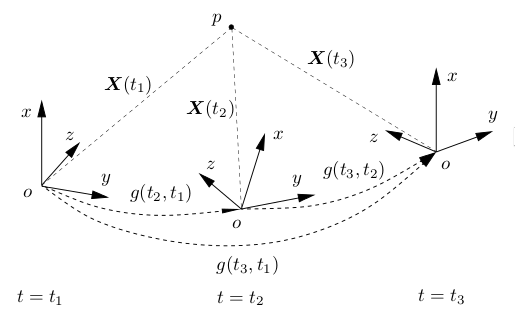
\includegraphics[scale=0.5]{rys3.png}
\end{center}

Ruch między kamerą w $t_3$ a kamerą w $t_2$ oznaczamy $g(t_3,t_2)$ a między kamerą w $t_3$ a $t_1$ oznaczamy $g(t_3,t_1)$. Mamy wtedy następującą zależność między współrzędnymi:

\begin{equation}
X(t_3)=g(t_3,t_2)X(t_2)=g(t_3,t_2)g(t_2,t_1)X(t_1)
\end{equation}

\noindent przyrównując to do bezpośredniej relacji między współrzędnymi w czasie $t_3$ a $t_1$:

\begin{equation}
X(t_3)=g(t_3,t_1)X(t_1)
\end{equation}


\noindent widzimy że zachowana jest następująca zasada:

\begin{equation}
g(t_3,t_1) = g(t_3,t_2)g(t_2,t_1)
\end{equation}

Zasada złożenia opisuje współrzędne $X$ punktu $p$ relatywnie do każdej pozycji kamery. Implikacją tej zasady jest również zasada inwersji:

\begin{equation}
g^{-1}(t_2,t_1)=g(t_1,t_2)
\end{equation}

\noindent gdyż $g(t_2,t_1)g(t_1,t_2)=g(t_2,t_2)=I$.

W przypadku gdy czas nie ma dla nas dużego znaczenia, możemy zamienić oznaczenie $g(t_i,t_j)$ na $g_{ij}$. Powyższe zasady zapisujemy wtedy jako:

\begin{equation}
X_i=g_{ij}X_j, \quad g_{ik}=g_{ij}g_{jk}, \quad g^{-1}_{ij}=g_{ji}
\end{equation}

\subsection{Zasady transformacji prędkości}

Rozumiejąc już jak działa transformacja współrzędnych, należy teraz przestudiować jaki ma ona wpływ na prędkość. Wiemy, że współrzędne $X(t)$ punktu $p \in \E^3$ względem do ruszającej się kamery są funkcją od czasu $t$:

\begin{equation}
X(t)=g_{wc}(t)X_0
\end{equation}

oraz prędkość w punkcie $p$ chwilowego układu kamery jest:

\begin{equation}
\dot{X}(t)=\dot{g}_{cw}(t)X_0
\end{equation}

Aby wyrazić $\dot{X}(t)$ w formie wartości ruszającego się układu zamienimy $X_0$ na $g_{cw}^{-1}X(t)$ i używając notacji skrętu zdefiniujemy:

\begin{equation}
\hat{V}^c_{cw}=\dot{g}_{cw}(t)g^{-1}_{cw}(t) \in se(3)
\end{equation}

\noindent Co można jeszcze inaczej zapisać jako

\begin{equation}
\dot{X}(t) = \hat{V}^c_{cw}(t)X(t)
\end{equation}

\noindent z tego że $\hat{V}^c_{cw}(t)$ jest postaci

\begin{equation}
\hat{V}^c_{cw}(t)= \begin{bmatrix} \hat{\omega}(t) & v(t) \\ 0 & 0 \end{bmatrix}
\end{equation}

\noindent Możemy przepisać prędkość punktu w przestrzeni 3d (zamiast współrzędnych jednorodnych) jako:

\begin{equation}
\dot{X}(t) = \hat{\omega}(t)X(t) + v(t)
\end{equation}

Fizyczną interpretacją sybolu $\hat{V}^c_{cw}$ jest prędkość układu globalnego ruszającego się względnie do układu kamery, potrząc z widoku kamery. Zwykle, by jasno ustalić fizyczne znaczenie prędkości, musimy podać prędkość którego układu rusza się względem którego, i z którego układu patrzymy. Jeśli zmienimy pozycję, z której obserwujemy prędkość, wyrażenie zmienia się wraz ze zmianą widoku. Np. załóżmy że obserwator jest w innym układzie współrzędnych przemieszczonych względem układu kamery poprzez ruch bryły sztywnej $g \in SE(3)$. Wtedy współrzędne tego samego punktu $p$ względem tego układu są $Y(t) = gX(t)$. Wyznaczamy prędkość w nowych układzie i otrzymujemy:

\begin{equation}
\dot{Y}(t)=g\dot{g}_{cw}(t)g^{-1}_{cw}(t)g^{-1}Y(t)=g\hat{V}^c_{cw}g^{-1}Y(t)
\end{equation}

\noindent Więc nowa prędkość (skręt) jest

\begin{equation}
\hat{V}=g\hat{V}^c_{cw}g^{-1}
\end{equation}

To jest ta sama wartość fizyczna ale obserwowana z innego punktu widokowego. Widzimy, że prędkości są połączone funkcją zdefiniowaną przez ruch $g$:

\begin{equation}
ad_g : se(3) \rightarrow se(3); \quad \hat{\xi} \rightarrow g\hat{\xi}g^{-1}
\end{equation}

To jest tzw. funkcja sprzężenia w przestrzeni $se(3)$. Używając tej notacji w poprzednim przykładzie mamy $\hat{V} = ad_g(\hat{V}^c_{cw})$. Zauważmy, że sprzężenie przekształca prędkość z jednego układu do drugiego. Wykorzystując fakt że $g_{cw}(t)g_{wc}(t)=I$ oczywistym jest, iż:

\begin{equation}
\hat{V}^c_{cw}=\dot{g}_{cw}g^{-1}_{cw}= -g^{-1}_{wc}\dot{g}_{wc}= -g_{cw}(\dot{g}_{wc}g^{-1}_{wc})g^{-1}_{cw}=ad_{g_{cw}}(-\hat{V}^w_{wc})
\end{equation}

\noindent więc $\hat{V}^c_{cw}$ można interpretować jako negację prędkości kamery ruszającej się względem układu globalnego, patrząc z układu kamery.

\end{document}
